\documentclass{standalone}

\usepackage{style}
\usepackage{tikz}
\usetikzlibrary{arrows}

\begin{document}
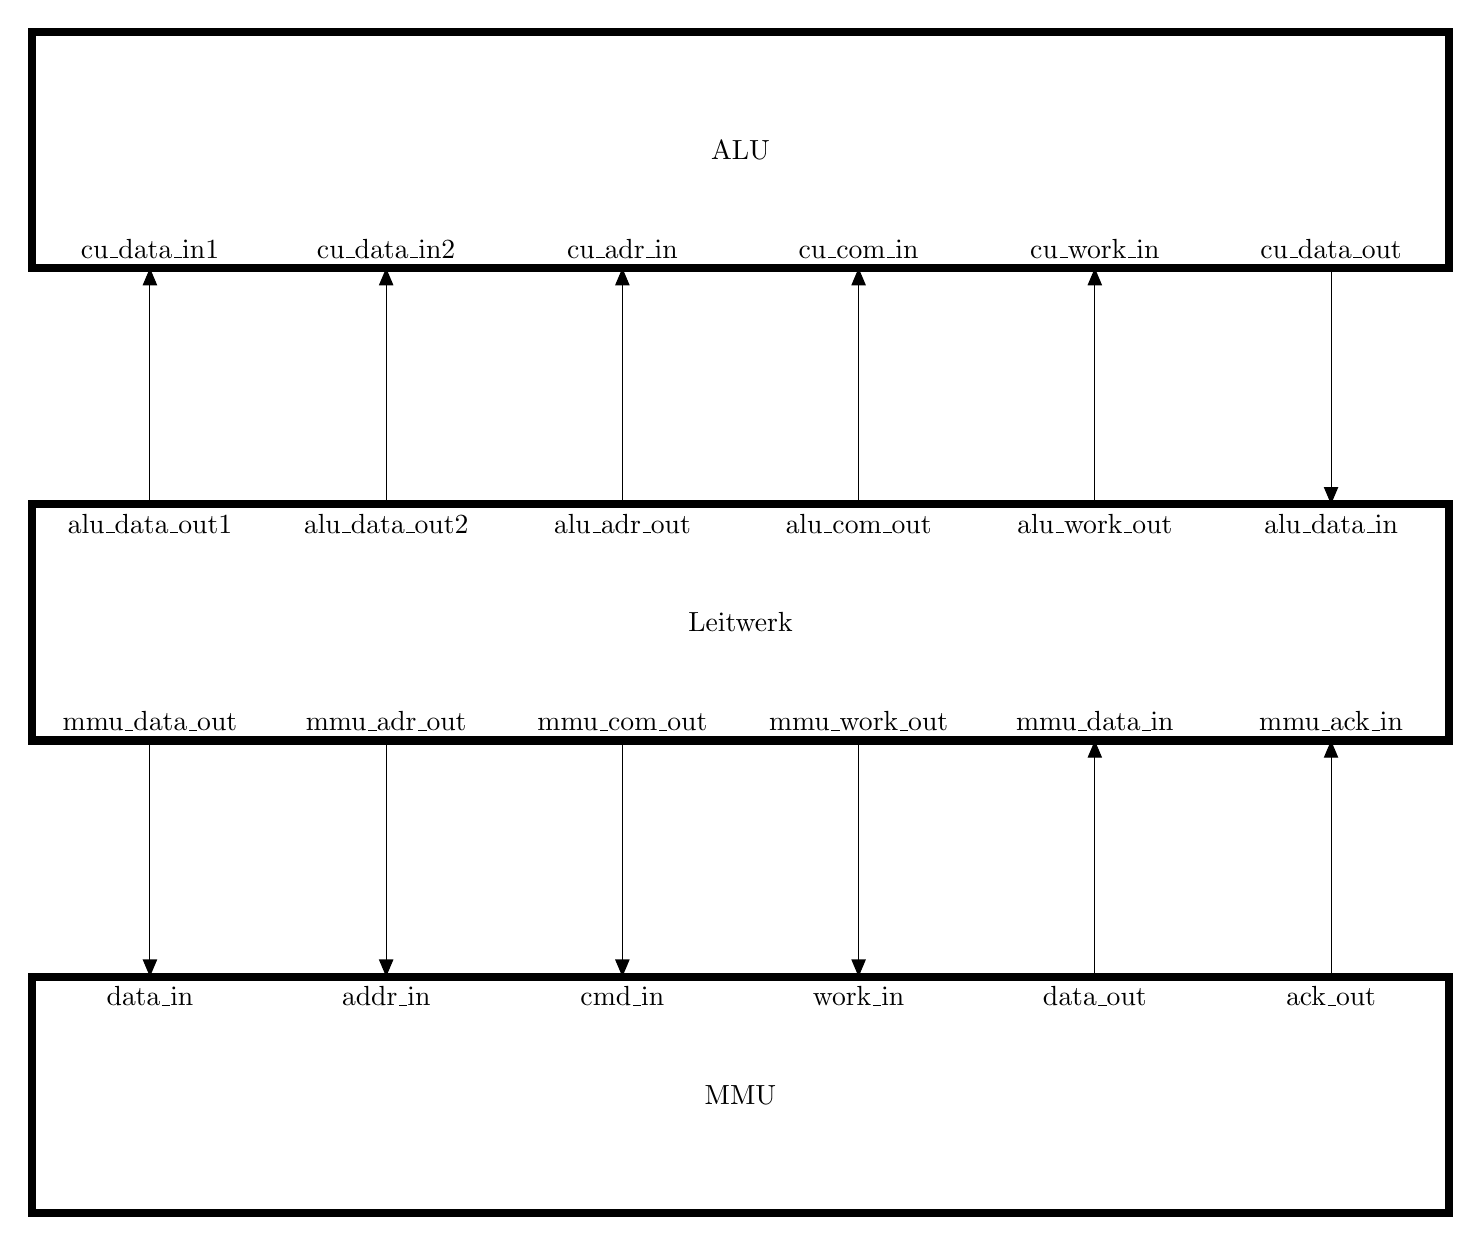
\begin{tikzpicture}[>=triangle 45]
\draw[line width=3pt] (0,0) rectangle node {ALU} (18,3);
\draw[->] (1.5,-3) node[below] {\Vhdl{alu\_data\_out1}} -- (1.5,0) node[above] {\Vhdl{cu\_data\_in1}};
\draw[->] (4.5,-3) node[below] {\Vhdl{alu\_data\_out2}} -- (4.5,0) node[above] {\Vhdl{cu\_data\_in2}};
\draw[->] (7.5,-3) node[below] {\Vhdl{alu\_adr\_out}} -- (7.5,0) node[above] {\Vhdl{cu\_adr\_in}};
\draw[->] (10.5,-3) node[below] {\Vhdl{alu\_com\_out}} -- (10.5,0) node[above] {\Vhdl{cu\_com\_in}};
\draw[->] (13.5,-3) node[below] {\Vhdl{alu\_work\_out}} -- (13.5,0) node[above] {\Vhdl{cu\_work\_in}};
\draw[<-] (16.5,-3) node[below] {\Vhdl{alu\_data\_in}} -- (16.5,0) node[above] {\Vhdl{cu\_data\_out}};
\draw[line width=3pt] (0,-3) rectangle node {Leitwerk} (18,-6);
\draw[<-] (1.5,-9) node[below] {\Vhdl{data\_in}} -- (1.5,-6) node[above] {\Vhdl{mmu\_data\_out}};
\draw[<-] (4.5,-9) node[below] {\Vhdl{addr\_in}} -- (4.5,-6) node[above] {\Vhdl{mmu\_adr\_out}};
\draw[<-] (7.5,-9) node[below] {\Vhdl{cmd\_in}} -- (7.5,-6) node[above] {\Vhdl{mmu\_com\_out}};
\draw[<-] (10.5,-9) node[below] {\Vhdl{work\_in}} -- (10.5,-6) node[above] {\Vhdl{mmu\_work\_out}};
\draw[->] (13.5,-9) node[below] {\Vhdl{data\_out}} -- (13.5,-6) node[above] {\Vhdl{mmu\_data\_in}};
\draw[->] (16.5,-9) node[below] {\Vhdl{ack\_out}} -- (16.5,-6) node[above] {\Vhdl{mmu\_ack\_in}};
\draw[line width=3pt] (0,-9) rectangle node {MMU} (18,-12);
\end{tikzpicture}
\end{document}

